\documentclass[12pt]{article}
\usepackage[english,thai]{babel}
\usepackage[utf8x]{inputenc}
\usepackage{listings}
\usepackage{xcolor}
\usepackage{graphicx}
\graphicspath{ {./images/} }
\usepackage{subcaption}
\usepackage{float}

\definecolor{codegreen}{rgb}{0,0.6,0}
\definecolor{codegray}{rgb}{0.5,0.5,0.5}
\definecolor{codepurple}{rgb}{0.58,0,0.82}
\definecolor{backcolour}{rgb}{0.95,0.95,0.92}
\lstdefinestyle{mystyle}{
    backgroundcolor=\color{backcolour},   
    commentstyle=\color{codegreen},
    keywordstyle=\color{magenta},
    numberstyle=\tiny\color{codegray},
    stringstyle=\color{codepurple},
    basicstyle=\ttfamily\footnotesize,
    breakatwhitespace=false,         
    breaklines=true,                 
    captionpos=b,                    
    keepspaces=true,                 
    numbers=left,                    
    numbersep=5pt,                  
    showspaces=false,                
    showstringspaces=false,
    showtabs=false,                  
    tabsize=2
}
\lstset{style=mystyle}

\title{Page repacement algorithms}

\begin{document}
\begin{center}
 \Huge
\textbf{Page repacement algorithms}

\textbf{Operating System}

\vspace{1.5cm}

\textbf{วสุธันย์ กิติจีราพัฒน์ (600610773)}
  
\end{center}

\newpage
\section{Page replacement algorithm}
\subsection{First in First Out (FIFO)}
นำข้อมูลเข้าสู้หน่วยความจำโดยใส่ไปที่ด้านท้ายของ list ทำให้ข้อมูลที่อยู่หน้าสุดเป็นตัวที่เข้ามาก่อน การนำ page ออกโดยดึง page ที่ิอยู่หน้าสุดออก
\lstinputlisting[language=Python, firstline=2, lastline=15]{algorithm.py}

\newpage
\subsection{Least Recently Used (LRU)}
เป็น algorithm ที่ดึงเอา page ที่อยู่นานที่สุดออก โดยบันทึกเวลาหน้าที่ถูกอ้างอิงไว้ล่าสุด แล้วเลือกหน้าที่ไม่ให้ถูกเรียกใช้นานที่สุดออก  


\lstinputlisting[language=Python, firstline=18, lastline=27]{algorithm.py}
\lstinputlisting[language=Python, firstline=35, lastline=57]{algorithm.py}

\subsection{Optimal Algorithm}
เป็น algorithm ที่สับเปลี่ยนหน้าที่ไม่ถูกใช้งานในอนาคตอันใกล้ และหน้าที่ไม่ได้ถูกใช้งานนานที่สุด
\lstinputlisting[language=Python, firstline=18, lastline=27]{algorithm.py}
\lstinputlisting[language=Python, firstline=29, lastline=59]{algorithm.py}


\newpage
\section{การทดลอง}
\subsection{แผนการทดลอง}
\paragraph{ทดลองโดยการสุ่มเลขช่วงๆ หนึ่งตามที่ต้องการ ซ้ำๆกันจำนวนหนึ่ง แล้วนำมาทดสอบเพื่อดู page faults ของแต่ละ algorithm ดังนี้}
\subsection{ผลการทดลอง}

\begin{figure}[H]
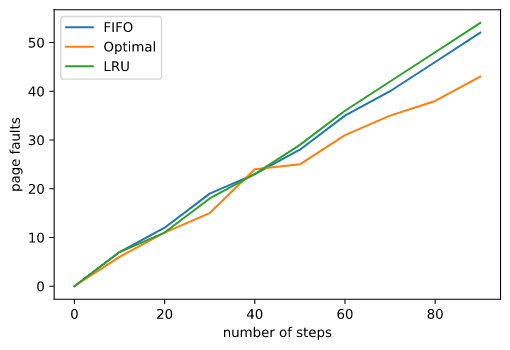
\includegraphics[width=\textwidth]{1.png}
ทดลองโดยสุ่ม reference string 100 ตัว Range ของการสุ่มคือเลข 0-9 ขนาดของ Page คือ 4 frame
\end{figure}

\begin{figure}[H]
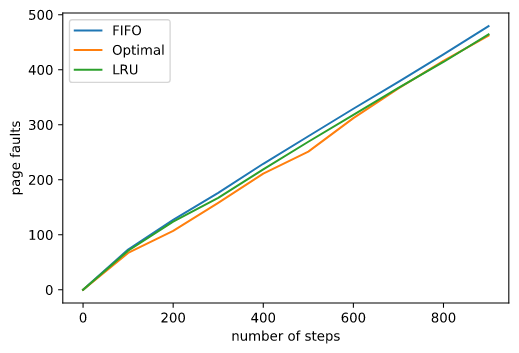
\includegraphics[width=\textwidth]{2.png}
ทดลองโดยสุ่ม reference string 1000 ตัว Range ของการสุ่มคือเลข 0-99 ขนาดของ Page คือ 50 frame
\end{figure}

\begin{figure}[H]
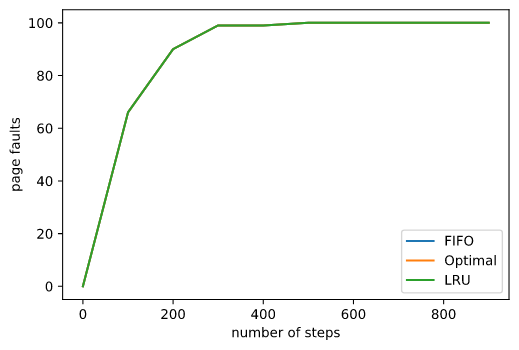
\includegraphics[width=\textwidth]{3.png}
ทดลองโดยสุ่ม reference string 1000 ตัว Range ของการสุ่มคือเลข 0-90 ขนาดของ Page คือ 100 frame
\end{figure}

\begin{figure}[H]
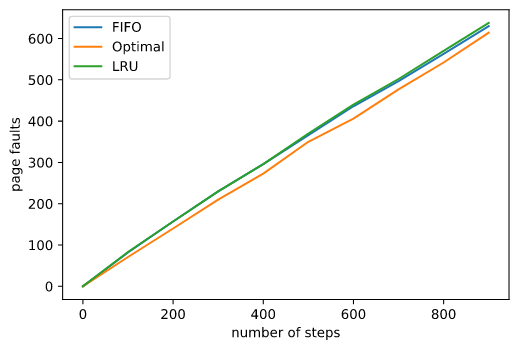
\includegraphics[width=\textwidth]{4.png}
ทดลองโดยสุ่ม reference string 1000 ตัว Range ของการสุ่มคือเลข 0-99 ขนาดของ Page คือ 30 frame
\end{figure}

\subsection{สรุปผลการทดลอง}
\paragraph{Page faults จะเกิดในรูปแบบของ linear ถ้า frame น้อยกว่า range ของการสุ่ม โดยที่ Optimal จะมีประสิทธิภาพมากที่สุด แต่ FIFO และ LRU จะใหล้เคียงกันแล้วแต่รูปแบบของข้อมูล}

\section{Reference}
\paragraph{Github: https://github.com/mrkwskiti/os-page-replacment}
\end{document}
